\documentclass[letterpaper,11pt]{article}
\usepackage[margin=1 in]{geometry}
%\usepackage{amsfonts}
\usepackage[pdftex]{graphicx}
%\usepackage[small,bf,sf,textfont={small,sf,bf}]{caption}
\usepackage{amssymb}
\usepackage{amsmath}
\usepackage{bm}
\usepackage[square,sort,comma,numbers]{natbib}
\usepackage{color}
\usepackage{algorithmicx}
\usepackage{algorithm}
\usepackage[noend]{algpseudocode}
\usepackage[shortlabels]{enumitem}
\usepackage{amsthm}
\newtheorem{thm}{Theorem}
\usepackage{tikz}
\usetikzlibrary{shapes,arrows,calc,positioning}
\usepackage{subfig}
\graphicspath{ {figures/} }
\def\signline{%
    \leftline{\hbox to 0in{}\hrulefill} % 26 Aug 2001	cwm
    }
%\author{Xueying Lu}  	% Required

%\address{201 E 24 St. POB 5.304\\ Austin, Texas 78712}  % Required

%\title{Efficient Algorithms for Coupled Flow and Poromechanics for Porous Media Applications}
% Required
%\supervisor
%	[Mary F. Wheeler]
%\committeemembers
%        [Mukul Sharma]
%        [Masa Prodanovic]
%        [Irene Gamba]
%\previousdegrees{B.S.}
\tikzstyle{decision} = [diamond, draw, aspect =2, text badly centered,
node distance = 0.2 in, inner sep =0 pt]
\tikzstyle{block} =[rectangle, draw, text width =4 in, text centered,node distance = 0.2 in, minimum height = 0.2 in]
\tikzstyle{smallblock} =[rectangle, draw, text width =1.5 in, text centered,node distance = 0.2 in, minimum height = 0.2 in]
\tikzstyle{line} =[draw, -latex']




\title{Parallel Implementation of Three-Way Coupling of Porous Media Flow and Mechanics}
\author{Xueying Lu,   xl4888}
%\institute{PCSE 2019 Spring Final Project}
%%%%%%%%%%%%%%%%%%%%%%%%%%%%%%%%%%%%%%%%%%%%%%%%%%%%%%%%%%%%%%%%%%%%%%
%	Macros.							     %
%%%%%%%%%%%%%%%%%%%%%%%%%%%%%%%%%%%%%%%%%%%%%%%%%%%%%%%%%%%%%%%%%%%%%%
%
%	Here some macros that are needed in this document:


\newcommand{\latexe}{{\LaTeX\kern.125em2%
                      \lower.5ex\hbox{$\varepsilon$}}}

\newcommand{\amslatex}{\AmS-\LaTeX{}}

\begin{document}
 %\commcertpage
 \maketitle 
\begin{abstract}
Coupled porous media flow and mechanics has numerous important applications in many disciplines of science and engineering. For example, in environmental engineering coupled flow and mechanics model is critical to the long-term accurate prediction of CO$_2$ sequestration. In field scale simulations of CO$_2$ storage, the coupled flow and mechanics systems are usually solved via fixed-stress iterative split. This decoupling algorithm enjoys the flexibility of choosing different discretization schemes and selecting different linear solver for each physics model. However field scale simulations are still computationally expensive and most of the computational time is attributed to the geomechanics update. Recently \citet{lu2019optimal} presented a three-way coupling algorithm for flow and mechanics, where an error indicator is calculated at the beginning of each time step to determine whether mechanics update is needed and whether fixed-stress iterative coupling is required. Numerical benchmarks shown that three-way coupling can significantly reduce computational time while maintain the same order of accuracy as of fixed-stress split. In this report we discuss the parallel implementation of three-way coupling based on MPI and show weak scaling performance.
\end{abstract}

 \section{Governing Equations}
 We use Biot's consolidation model for a linear elastic, homogeneous, isotropic porous medium saturated with a slightly compressible fluid. The model is based on a quasi-static assumption, namely it assumes that the material deformation rate is much slower than the flow rate and hence the second order derivative of the displacement is zero. We then summarize the governing equations for linearized single phase flow in linear poroelastic medium as follows:
\begin{equation}\label{eq:sum-1}
    -\nabla \cdot (\lambda (\nabla \cdot \bm{u})\bm{I}+2\mu\bm{\epsilon}(\bm{u}) -\alpha p \bm{I}) = \bm{f}
\end{equation}
\begin{equation}
    \frac{\partial}{\partial t}\left( 
    \frac{1}{M} p+\alpha \nabla \cdot \bm{u} \right)-\frac{1}{\mu_f} \nabla \cdot (\bm{\kappa}\nabla (p-\rho_{f,r}g\eta))=q
\end{equation}
\begin{align}
    p(t)=g(t) \text{ on } \Gamma^p_D\\
    -\bm{\kappa} \frac{1}{\mu_f}(\nabla p -\rho_{f,r} g\nabla \eta)\cdot \bm{n} =0 \text{ on }\Gamma^p_N\\
    \bm{u}(t) = 0 \text{ on } \Gamma^u_D\\
    \bm{\sigma}^T\bm{n}_N=\bm{t}_N \text{ on } \Gamma^u_N\\
    p(0) =p_0\\
    \bm{u}(0)=\bm{0}\label{eq:sum-last}
\end{align}
$\alpha$ is the Biot parameter, $\rho_s$ is the solid density, $\rho_f$ is the fluid density and $\phi$ is the porosity. $\bm{\sigma}$ is the total stress tensor, $\bm{I}$ is the identity tensor, $p$ is the pore pressure. $q$ is the volumetric sink/source term.

\section{Decoupling Schemes}
\subsection{Fixed-stress iterative split}
We summarize the fixed-stress iterative split in Figure \ref{fig:fixed-stress}.
\begin{figure}[h!]
\begin{center}
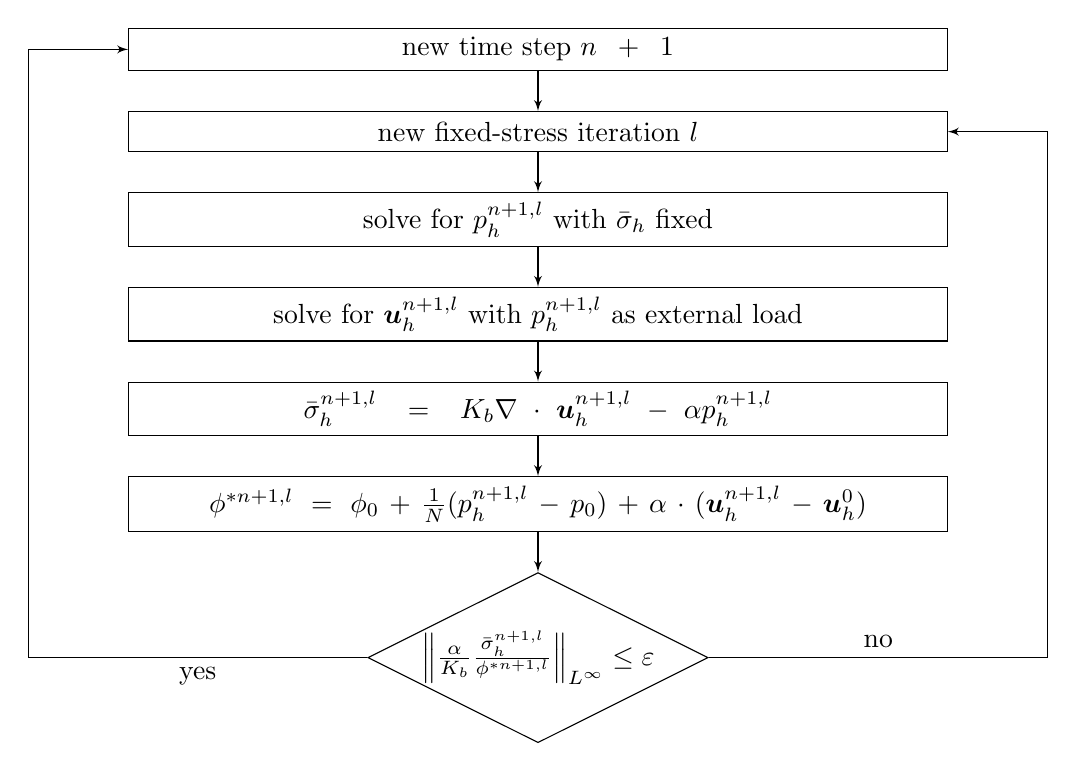
\begin{tikzpicture}[node distance = 2cm, auto]

\node [block] (init) {new time step $n+1$};
\node [block, below = of init] (fixed) {new fixed-stress iteration $l$};
\node [block, below = of fixed] (flow){solve for $p_h^{n+1,l}$ with $\bar{\sigma}_h$ fixed};
\node [block, below =of flow] (mechanics) {solve for $\bm{u}_h^{n+1,l}$ with $p_h^{n+1,l}$ as external load};
\node [block, below = of mechanics] (meanstress) {$\bar{\sigma}_h^{n+1,l}=K_b\nabla\cdot \bm{u}^{n+1,l}_h-\alpha p_h^{n+1,l}$};
\node [block, below = of meanstress] (porosity){$\phi^{*n+1,l}=\phi_0+\frac{1}{N}(p_h^{n+1,l}-p_0)+\alpha\cdot (\bm{u}_h^{n+1,l}-\bm{u}_h^0)$};
\node [decision, below = of porosity] (converge)% {$\left\Vert \frac{\tilde{\phi}^{*n+1,l}-\phi^{*n+1,l}}{\phi^{*n+1,l}}\right\Vert_L^\infty <\varepsilon$};
{$\left\Vert \frac{\alpha}{K_b}\frac{\bar{\sigma}_h^{n+1,l}}{\phi^{*n+1,l}}\right\Vert_{L^\infty}\leq \varepsilon$};
\coordinate (left new step) at ($(init.west) - (0.5 in, 0)$);
\coordinate (right fixed) at ($(fixed.east) +(0.5 in, 0)$);
\path [line] (init) -- (fixed);
\path [line] (fixed) -- (flow);
\path [line] (flow) -- (mechanics);
\path [line] (mechanics) -- (meanstress);
\path [line] (meanstress) -- (porosity);
\path [line] (porosity) --(converge);
\path [line] (converge.west) -| node [near start] {yes} (left new step) -- (init.west);
\path [line] (converge.east) -| node [near start] {no} (right fixed) -- (fixed.east);
\end{tikzpicture}
\end{center}
\caption{Flow chart of fixed-stress iterative coupling of flow and mechanics}\label{fig:fixed-stress}
\end{figure}

\subsection{Three-way coupling}
\begin{figure}[h!]
\begin{center}
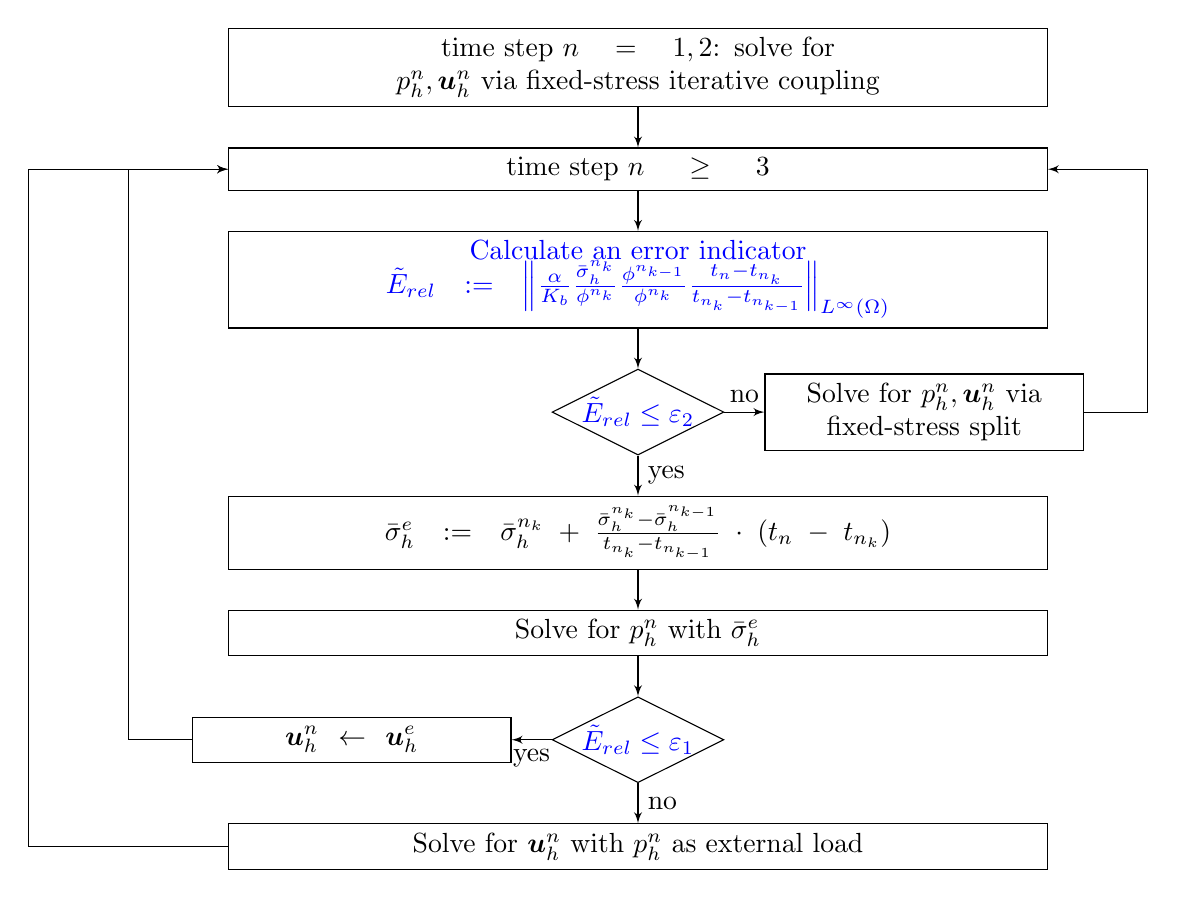
\begin{tikzpicture}[node distance = 2cm, auto]
\node [block] (init) {time step $n=1,2$: solve for $p_h^n,\bm{u}_h^n$ via fixed-stress iterative coupling};
\node [block, below = of init] (newstep) {time step $n\geq 3$};
\node [block, below = of newstep] (error) {\color{blue} Calculate an error indicator\\$ \tilde{E}_{rel}:= \left\Vert \frac{\alpha}{K_b}\frac{\bar{\sigma}_h^{n_k}}{\phi^{n_k}}\frac{\phi^{n_{k-1}}}{\phi^{n_k}}\frac{t_n-t_{n_k}}{t_{n_k}-t_{n_{k-1}}}\right\Vert_{L^\infty(\Omega)}$};
\node [decision, below = of error] (eps2) {\color{blue}$\tilde{E}_{rel}\leq \varepsilon_2$};
\node [smallblock, right = of eps2] (solve){Solve for $p_h^{n},\bm{u}_h^n$ via fixed-stress split};
\node [block, below = of eps2] (extrapolate){$\bar{\sigma}_h^e:=\bar{\sigma}_h^{n_k}+\frac{\bar{\sigma}_h^{n_k}-\bar{\sigma}_h^{n_{k-1}}}{t_{n_k}-t_{n_{k-1}}}\cdot (t_n-t_{n_k})$};
\node [block, below = of extrapolate] (flow) {Solve for $p_h^{n}$ with $\bar{\sigma}_h^e$};
\node [decision, below = of flow] (eps1) {\color{blue}$\tilde{E}_{rel}\leq \varepsilon_1$};
\node [smallblock, left = of eps1] (skip){$\bm{u}_h^n\gets \bm{u}_h^e$};
\node [block, below = of eps1] (explicit) {Solve for $\bm{u}_h^n$ with $p_h^n$ as external load};

\path [line] (init) -- (newstep);
\path [line] (newstep) -- (error);
\path [line] (error) --(eps2);
\path [line] (eps2) -- node {yes}(extrapolate);
\path [line] (eps2) -- node {no}(solve);
\path [line] (extrapolate) -- (flow);
\path [line] (flow) -- (eps1);
\path [line] (eps1) -- node {yes}(skip);
\path [line] (eps1) -- node {no}(explicit);

\coordinate (l1) at ($(newstep.west) - (0.5 in, 0)$);
\coordinate (r1) at ($(newstep.east) + (0.5 in, 0)$);
\coordinate (l2) at ($(newstep.west) - (1 in, 0)$);
\path [line] (skip) -| (l1) -- (newstep.west);
\path [line] (explicit) -| (l2) -- (newstep.west);
\path [line] (solve) -| (r1) --(newstep.east);
\end{tikzpicture}
\end{center}
\caption{Flow chart for three-way coupling}\label{fig:three-way}
\end{figure}

\section{Parallel Implementation of Three-Way Coupling}
The implementation of three-way coupling is build upon existing parallel implementations for flow and mechanics problems. Namely we need to parallel the steps colored in blue in Figure \ref{fig:three-way}.

\begin{algorithm}
\caption{Parallel Implementation of Three-Way Coupling}\label{algo:parallel}
\begin{algorithmic}[1]

\State Calculate error indicator $\tilde{E}_{rel}$
\State Get the maximum $\tilde{E}_{rel}$ across all processors by MPI\_Reduce \\
\texttt{call MPI\_Reduce(Erel, MaxErel, 1, MPI\_REAL8, MPI\_MAX,root, MPI\_COMM\_WORLD,ierr);}
\If{\texttt{MYPRC==root}}
\State \texttt{COUPLING\_TYPE=0}
\If{\texttt{MaxErel}  $<\varepsilon_1$} \State \texttt{COUPLING\_TYPE=2}
\ElsIf{\texttt{MaxErel}  $<\varepsilon_1$} \State \texttt{COUPLING\_TYPE=1}
\EndIf
\EndIf
\State Broadcast  \texttt{COUPLING\_TYPE} to all processors\\
\texttt{call MPI\_Bcast(COUPLING\_TYPE, 1, MPI\_INT,root, MPI\_COMM\_WORLD, ierr);}
\end{algorithmic}
\end{algorithm}
 \bibliographystyle{abbrvnat}
 \bibliography{proposal_ref}
 
\end{document}
